\documentclass[unknownkeysallowed]{beamer}
\usetheme{RJH}
\usepackage[orientation=portrait, size=a4, scale=0.6]{beamerposter}
\usepackage[absolute,overlay]{textpos}
\usepackage{graphicx}
\usepackage{epsfig}
\usepackage{hyperref}
\setlength{\TPHorizModule}{1cm}
\setlength{\TPVertModule}{1cm}
\title{Numerical methods in Astronomy - Python way}
\author{Z. Janak}
\footer{More information at janak@physics.muni.cz}
\date{}
\usepackage[czech]{babel}
%\usepackage[latin2]{inputenc} % pro iso8859-2
\usepackage[utf8]{inputenc}   % pro unicode UTF-8
%\usepackage[cp1250]{inputenc} % pro win1250
\begin{document}
\begin{frame}{} 

\begin{textblock}{9.75}(0.5,2)
\begin{block}{Motivation}
Through the study of the astrophysics, students are often exposed to the problem,
which must be solved using standard numerical methods, like optimalization, integration,
differentiation or Monte Carlo simulation. With the power of the PYTHON language and 
huge amount of the scientific libraries it is very often simple task. Unfortunately,
due to generally poor programming skill (not only in PYTHON) and knowledge of the students, 
sometimes students are not able to solve the problem. Developed lectures about numerical
 methods in astronomy is the way how to help him.
\end{block}

\begin{block}{Optimalization problem}
One of the typical task in analysis of the binary stars is derivation of the spectroscopic orbital parameters from the observations namely from the radial velocity curve fitting. Usually one can use method known as {\it differential corrections}, but for educational purpose we used genetical algorithms, which are more robust and result can be used as the first guess for the parameters. We used module PyPIKAIA, Python version
of the subroutine PIKAIA 
\begin{figure}
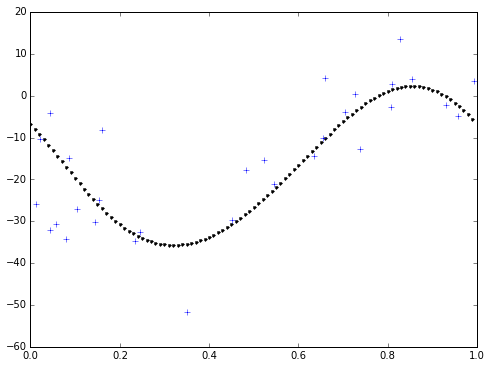
\includegraphics[width=1\textwidth, height=4cm]{radialvelocity.png}
\end{figure}
\end{block}
\end{textblock}

\begin{textblock}{9.5}(10.75,2)
\begin{block}{Hydrodynamics in cube}
Solution of the hydrodynamics equation in the various astrophysical configuration is one of the 
major problem in numerical astrophysics. For fast and power computing it is necessary to use different language instead of python. But for
simple problems and educational purposes PYTHON can be used very well. Basic principles of the computational fluid dynamics can be illustrated on the solution of the
Burgers equation, simple nonlinear advective equation. With the help of the interactive capabilities of the IPYTHON notebooks, students can 
easily explore influence of the parameters, like time or space steps, advective velocity or initial condiditions.
\end{block}

\begin{block}{References}
\bibliographystyle{alpha}
\bibliography{scipyposter}
\end{block}
\end{textblock}

\end{frame}
\end{document}

